\section{Extreme Points}\label{sec:mcov_chap2_sec3}
What we have seen so far is that satisfying the Euler-Lagrange equations is sufficient for being a critical point. That's okay, but we are more interested in extreme points, more precisely, minimizers. Maximizers can be treated analogously.\\[11pt]

\textbf{\underline{Definition 2.3.1}}\\
We consider an open, bounded set $\Omega\subset\mathbb{R}^d$ and $\emptyset\ne M\subset C^1(\Omega;\mathbb{R}^m)$. Let $I:M\longrightarrow\mathbb{R}\cup\{\pm\infty\}$. Then $u_0\in M$ is called
\begin{itemize}
	\item[(i)] \textit{weak local minimizer of $I$} if there is $\varepsilon>0$ such that for all $v\in M$ with $\lVert u_0-v\rVert_{C^1(\Omega)}\leq\varepsilon$ it holds $I(v)\geq I(u_0)$.
	\item[(ii)] \textit{strong local minimizer of $I$} if there is $\varepsilon>0$ such that for all $v\in M$ with $\lVert u_0-v\rVert_{C^0(\Omega)}\leq\varepsilon$ it holds $I(v)\geq I(u_0)$.
	\item[(iii)] \textit{global minimizer of $I$} if for all $v\in M$ we have $I(v)\geq I(u_0)$.\\[11pt]
\end{itemize}

\textbf{Remark 2.3.2}\\
We have the implications
\[\text{global minimizer}\quad\Rightarrow\quad\text{strong local minimizer}\quad\Rightarrow\quad\text{weak local minimizer}.\]
The first one is clear, and the second one follows because $\lVert\cdot\rVert_{C^0(\Omega)}\leq\lVert\cdot\rVert_{C^1(\Omega)}$, so for a weak local minimizer, $I(v)\geq I(u_0)$ has to be satisfied for a smaller class of functions $v$.\newpage

\hypertarget{example_2_3_3}{\textbf{Example 2.3.3}}\\
(Weak vs. strong minimizers)\\
Consider
\[I(u)=\int_0^1{(1-(u'(x))^2)^2\mathrm{d}x}\]
on $M=M_a:=\{u\in C^1([0,1])\mid u(0)=0,u(1)=a\}$ with parameter $a\geq0$. The volume density for $I$ is $f(A)=(1-A^2)^2$ and thus independent of $x$ and $u$.

\begin{figure}[ht]
	\centering
	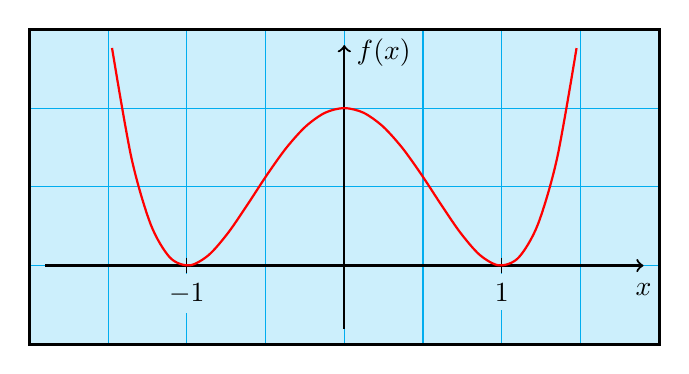
\begin{tikzpicture}
		% Hintergrund
		\fill[cyan!20] (-4, -1) rectangle (4, 3);
		\draw[cyan, step=1] (-4, -1) grid (4, 3);

		% Achsen
		\draw[thick, ->] (-3.8, 0) -- (3.8, 0);
		\node at (3.8, -0.3) {$x$};
		\draw[thick, ->] (0, -0.8) -- (0, 2.8);
		\node at (0.5, 2.7) {$f(x)$};
		\draw[thin] (-2, 0.1) -- (-2, -0.1) node[below, fill=cyan!20] {$-1$};
		\draw[thin] (2, 0.1) -- (2, -0.1) node[below, fill=cyan!20] {$1$};

		% Funktion
		\draw[thick, red] plot[smooth, domain=-2.95:2.95] (\x, {2*(1-(\x/2)^2)^2});

		% Rahmen
		\draw[very thick] (-4, -1) rectangle (4, 3);
	\end{tikzpicture}
	\caption{Graph of volume density $f$.}
\end{figure}

To set up the Euler-Lagrange equations (EL), we need to compute the derivatives. It holds $\partial_Af(u')=-4u'(1-(u')^2)$ and $\partial_uf(u')=0$, so (EL) is just
\[0=[4u'(1-(u'))^2]'.\]
That's a second-order ordinary differential equation again, so not easy. Thus, we apply Noether's theorem again. Even both statements, \hyperlink{lemma_2_2_13}{Lemma 2.2.13 (a), (b)} are applicable here. We obtain:
\begin{itemize}
	\item[(a)] $\partial_Af(u')=-4u'(1-(u')^2)$ is constant in $x$.
	\item[(b)] $u'\partial_Af(u')-f(u')=-4(u')^2(1-(u')^2)-(1-(u')^2)^2=(-1-3(u')^2)(1-(u')^2)$ is constant in $x$.
\end{itemize}
With that one can find with algebraic arguments that $u'$ has to be constant. This leads to $u_a(x)=ax$ which indeed is a critical point. Now we want to analyze whether $u_a$ is a minimizer in some sense. For $w\in C_0^1([0,1])$ we have via a Taylor expansion of $f$ at $u_a'$
\begin{align*}
	I(u_a+w)&=\int_0^1{f(u_a'(x)+w'(x))\mathrm{d}x}\\
	&=I(u_a)+f'(a)\underbrace{\int_0^1{w'(x)\mathrm{d}x}}_{=w(1)-w(0)=0}+\frac{1}{2}f''(a)\int_0^1{(w'(x))^2\mathrm{d}x}\\
	&\qquad\qquad+\frac{1}{6}f'''(a)\int_0^1{(w'(x))^3\mathrm{d}x}+\frac{1}{24}f''''(a)\int_0^1{(w'(x))^4\mathrm{d}x}.
\end{align*}
The derivatives of $f$ are
\begin{align*}
	f(A)&=(1-A^2)^2\\
	f'(A)&=-4A(1-A^2)\\
	f''(A)&=12A^2-4\\
	f'''(A)&=24A\\
	f''''(A)&=24.
\end{align*}
It turns out that the existence and type of minimizers depend on $a$.
\begin{itemize}
	\item[(A)] Let $\lvert a\rvert\geq1$. For general $\xi\in\mathbb{R}$ we have
	\[\frac{1}{2}f''(a)\xi^2+\frac{1}{6}f'''(a)\xi^3+\frac{1}{24}f''''(a)\xi^4=\xi^2\underbrace{(6a^2-2+4a\xi+\xi^2)}_{=(\xi+2a)^2+2a^2-2\geq0}\geq0,\]
	so $I(u_a+w)\geq I(u_a)$ for all $w\in C_0^1([0,1])$, i.e. $I(w)\geq I(u_a)$ for all $w\in M_a$. Hence, $u_a$ is a global minimizer.
	\item[(B)] Let $\frac{1}{\sqrt{3}}<\lvert a\rvert<1$. We then have $f''(a)>0$ and thus
	\[I(u_a+w)\geq I(u_a)+\int_0^1{(w'(x))^2\underbrace{\left(\frac{1}{2}f''(a)-4a\varepsilon-\varepsilon^2\right)}_{>0\text{ for }\varepsilon>0\text{ small enough}}\mathrm{d}x}\geq I(u_a)\]
	for $w\in C_0^1([0,1])$ with $\lVert w\rVert_{C^1([0,1])}\leq\varepsilon$. This shows that $u_a$ is a weak local minimizer.\\

	But $u_a$ is not a strong local minimizer. To show this, we perturb $u_a$ by a zigzag function. So, what we actually need to show is that, for a suitable $c>0$, for all $n\in\mathbb{N}$ there exists $\widetilde{u}_n\in M_a$ with $\lVert\widetilde{u}_n-u_a\rVert_{C^0([0,1]}<\frac{c}{n}$ but $I(u_a)>I(\widetilde{u}_n)$. For that, take
	\[\hat{u}_n(x):=u_a(x)+w_n(x)\]
	with $w_n\in PC^1([0,1])$, $w_n(0)=w_n(1)=0$, such that $\hat{u}_n(x)'\in\{-1,1\}$ for each $x\in[0,1]$.\\

	\begin{figure}[ht]
		\centering
		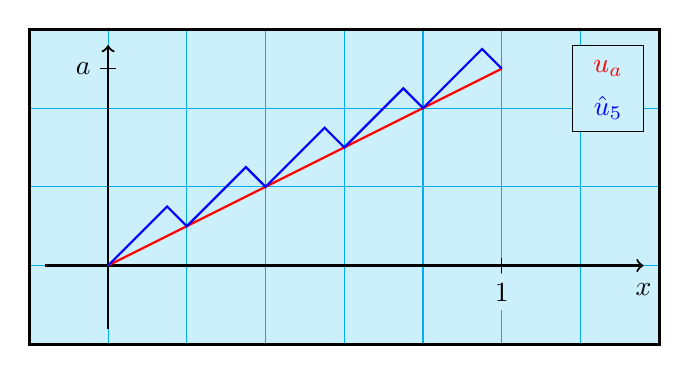
\begin{tikzpicture}
			% Hintergrund
			\fill[cyan!20] (-1, -1) rectangle (7, 3);
			\draw[cyan, step=1] (-1, -1) grid (7, 3);

			% Achsen
			\draw[thick, ->] (-0.8, 0) -- (6.8, 0);
			\node at (6.8, -0.3) {$x$};
			\draw[thick, ->] (0, -0.8) -- (0, 2.8);
			\draw[thin] (5, 0.1) -- (5, -0.1) node[below, fill=cyan!20] {$1$};
			\draw[thin] (0.1, 2.5) -- (-0.1, 2.5) node[left, fill=cyan!20] {$a$};

			% Legende
			\draw[fill=cyan!20] (5.9, 1.7) rectangle (6.8, 2.8);
			\node[red] at (6.35, 2.5) {$u_a$};
			\node[blue] at (6.35, 2) {$\hat{u}_5$};

			% Funktionen
			\draw[thick, red] (0, 0) -- (5, 2.5);
			\draw[thick, blue] (0, 0) -- (0.75, 0.75) -- (1, 0.5) -- (1.75, 1.25) -- (2, 1) -- (2.75, 1.75) -- (3, 1.5) -- (3.75, 2.25) -- (4, 2) -- (4.75, 2.75) -- (5, 2.5);

			% Rahmen
			\draw[very thick] (-1, -1) rectangle (7, 3);
		\end{tikzpicture}
		\caption{Illustration of $\hat{u}_n$ for $n=5$.}
	\end{figure}

	A possible choice could be
	\[w_1(x)=\left\{\begin{array}{rl}
		m_1x&\text{if }0\leq x\leq x_*,\\
		m_2(x-1)&\text{if }x_*<x\leq 1,
	\end{array}\right.\]
	where $x_*:=\frac{m_2}{m_2-m_1}$ so that $w_1$ is continuous, and the quantities $m_1,m_2$ should satisfy $m_1=1-a$, $m_2=-(1+a)$ so that $\hat{u}_n'(x)\in\{-1,1\}$ is guaranteed. Then extend $w_1$ periodically to $\mathbb{R}$ such that $w_1(x+1)=w_1(x)$, and define $w_n(x)=\frac{1}{n}w_1(nx)$ for all $x\in\mathbb{R}$. Then $w_n$ has period $\frac{1}{n}$ and amplitude $\sim\frac{1}{n}$. So
	\[\lVert\hat{u}_n-u_a\rVert_{C^0([0,1])}=\lVert w_n\rVert_{C^0([0,1])}=\frac{1}{n}\lVert w_1\rVert_{C^0([0,1])}\to0\]
	as $n\to\infty$, but $\hat{u}_n'(x)=a+w_n'(x)=\pm1$ for each $x\in[0,1]$ -- except at the $n$ kinks --, i.e. $I(\hat{u}_n)=0<I(u_a)$.\\

	But the problem is that $\hat{u}_n\in PC^1([0,1])\setminus C^1([0,1])$. We obtain our desired sequence $(\widetilde{u}_n)_{n\in\mathbb{N}}$ by smoothing the $n$ kinks $x_k$ of $\hat{u}_n$, which are
	\[x_k=\frac{1+a}{2n}+\frac{k}{n}\]
	for $k=0,\dotsc,n-1$. Smoothing $\hat{u}_n$ in a small $\delta$-neighbourhood of $x_k$ quadratically gives $\widetilde{u}_n\in C^1([0,1])$ with
	\begin{align*}
		I(\widetilde{u}_n)&=\sum_{k=0}^{n-1}{\int_{x_k-\delta}^{x_k+\delta}{(1-(\widetilde{u}_n'(x))^2)^2\mathrm{d}x}}\\
		&=\sum_{k=0}^{n-1}{\int_{x_k-\delta}^{x_k+\delta}{\underbrace{\left(1-\left(\frac{1}{\delta}(x_k-x)\right)^2\right)^2}_{\leq1}\mathrm{d}x}}\\
		&\leq 2n\delta.
	\end{align*}
	Choose $\delta=\delta_n=\frac{1}{n^2}$, then $I(\widetilde{u}_n)\to0$ as $n\to\infty$. Since $I(u_a)=(1-a^2)^2>0$ for $a\in(\frac{1}{\sqrt{3}},1)$, $u_a$ is not a strong minimizer.
	\item[(C)] Let $0\leq\lvert a\rvert\leq\frac{1}{\sqrt{3}}$.\\

	At first, consider $\lvert a\rvert<\frac{1}{\sqrt{3}}$. Then we have $f''(a)<0$. If we have a look at our Taylor expansion, then a natural idea would be to construct functions with somehow small derivative, so that the terms of third and fourth order have a relatively small contribution. We choose $w_\varepsilon(x)=\varepsilon\sin(\pi x)$. Then $w_\varepsilon(0)=0=w_\varepsilon(1)$, and $\lVert w_\varepsilon\rVert_{C^1([0,1])}\to0$ as $\varepsilon\to0$. We can estimate $\lvert\cos^3\rvert,\lvert\cos^4\rvert\leq1$ so that
	\[I(u_a+w_\varepsilon)\leq I(u_a)+\underbrace{\frac{1}{2}f''(a)\varepsilon^2\int_0^1{\pi^2(\cos(\pi x))^2\mathrm{d}x}}_{<0}+4a\varepsilon^3+\varepsilon^4<I(u_a)\]
	if $\varepsilon$ is sufficiently small. Hence, $u_a$ is no weak local minimizer.\\

	Now we consider $\lvert a\rvert=\frac{1}{\sqrt{3}}$. We only concentrate on the case $a=\frac{1}{\sqrt{3}}$; the other one can be treated in a similar way. So $f'''(a)=0$, hence
	\[I(u_a+w)=I(u_a)+\int_0^1{\frac{4}{\sqrt{3}}(w'(x))^3+(w'(x))^4\mathrm{d}x}.\]
	Again, we want to conclude that $u_a$ is not a weak local minimizer. To this end, we show there exists a sequence $(w_k)_{k\in\mathbb{N}}\subset C_0^1([0,1])$ such that $\lVert w_k\rVert_{C^1([0,1])}\to0$ as $k\to\infty$ and
	\[\int_0^1{\frac{4}{\sqrt{3}}(w'_k(x))^3+(w_k'(x))^4\mathrm{d}x}<0\]
	for all sufficiently large $k$. For that, define for $\gamma\in C_0^1([0,1])$ the function $w_k(x):=\frac{1}{k}\gamma(x)$ and choose $\gamma$ in such a way that
	\[\int_0^1{\frac{4}{k^3\sqrt{3}}(\gamma'(x))^3\mathrm{d}x}+\frac{1}{k^4}\int_0^1{(\gamma'(x))^4\mathrm{d}x}<0\]
	for large $k$. It is even sufficient to construct $\gamma$ such that $\int_0^1{(\gamma'(x))^3\mathrm{d}x}<0$. First we consider
	\[\hat{\gamma}:[0,1]\longrightarrow\mathbb{R},\qquad\hat{\gamma}(x):=\left\{\begin{array}{rl}
		x/\theta&\text{for }0\leq x<\theta,\\
		\frac{1-x}{1-\theta}&\text{for }\theta\leq x\leq 1,
	\end{array}\right.\]
	which is continuous, and let $\gamma$ then be a modification that is smooth in an $\varepsilon$-neighbourhood of $\theta$. Then we obtain
	\begin{align*}
		\int_0^1{(\gamma'(x))^3\mathrm{d}x}&=C_\varepsilon+\int_0^1{(\hat{\gamma}'(x))^3\mathrm{d}x}\\
		&=C_\varepsilon+\theta\frac{1}{\theta^3}+(1-\theta)\left(\frac{-1}{1-\theta}\right)^3\\
		&=C_\varepsilon+\frac{1}{\theta^2}-\frac{1}{(1-\theta)^2},
	\end{align*}
	where $C_\varepsilon$ denotes a perturbation term. But for $\varepsilon$ small and $\theta\in(1/2,1)$, we obtain $\int_0^1{(\gamma'(x))^3\mathrm{d}x}<0$.\\[11pt]
\end{itemize}

\hypertarget{theorem_2_3_4}{\textbf{\underline{Theorem 2.3.4}}}\\
(Local weak minimizers)\\
Let $f\in C^2(\Omega\times\mathbb{R}^m\times\mathbb{R}^{m\times d})$ and $g\in C^2(\partial\Omega\times\mathbb{R}^m)$.
\begin{itemize}
	\item[(i)] Necessary condition: If $u_*\in M$ is a weak local minimizer of $I:M\longrightarrow\mathbb{R}$, then for all $v\in X_0$ it holds $D^2I(u)[v]\geq0$.
	\item[(ii)] Sufficient condition: If $u_*\in M$ is a critical point of $I:M\longrightarrow\mathbb{R}$ and there exists $\gamma_*>0$ such that for all $v\in X_0$ it holds
	\[D^2I(u_*)[v]\geq\gamma_*\left(\int_\Omega{\lvert\nabla v(x)\rvert^2+\lvert v(x)\rvert^2\mathrm{d}x}+\int_{\partial\Omega}{\lvert v(x)\rvert^2\mathrm{d}a}\right),\]
	then $u_*$ is a strict weak local minimizer of $I$.\\
\end{itemize}

\textit{Proof:}
\begin{itemize}
	\item[(i)] By hypothesis, $t=0$ is a minimizer of $t\longmapsto I(u_*+tv)$ for all $v\in X_0$. Hence, by real Analysis,
	\[0\leq\left.\frac{\mathrm{d}^2}{\mathrm{d}t^2}I(u_*+tv)\right|_{t=0}=D^2I(u_*)[v].\]
	\item[(ii)] A Taylor expansion for $f$ and $g$ yields
	\begin{align*}
		f(\cdot,u_*+v,\nabla u_*+\nabla v)&=f(\cdot,u_*,\nabla u_*)+D_uf(\cdot,u_*,\nabla u_*)[v]+D_Af(\cdot,u_*,\nabla u_*)[\nabla v]\\
		&\qquad\qquad+\frac{1}{2}D_u^2f(\cdot,u_*,\nabla u_*)[v]+D_AD_uf(\cdot,u_*,\nabla u_*)[v,\nabla v]\\
		&\qquad\qquad+\frac{1}{2}D_A^2f(\cdot,u_*,\nabla u_*)[\nabla v]+r(\cdot,v,\nabla v)\\
		g(\cdot,u_*+v)&=g(\cdot,u_*)+D_ug(\cdot,u_*)[v]+\frac{1}{2}D_u^2g(\cdot,u_*)[v]+s(\cdot,v),
	\end{align*}
	where $r(x,u,A)=o(\lvert A\rvert^2+\lvert u\rvert^2)$ and $s(x,u)=o(\lvert u\rvert^2)$ uniformly in $\overline{\Omega}$ and $\partial\Omega$, respectively. Then \hyperlink{lemma_2_2_4}{Lemma 2.2.4} yields
	\begin{align*}
		I(u_*+u)&=I(u_*)+\underbrace{DI(u_*)[v]}_{=0}+\frac{1}{2}D^2I(u_*)[v]\\
		&\qquad\qquad+\int_\Omega{r(x,v(x),\nabla v(x))\mathrm{d}x}+\int_{\partial\Omega}{s(x,v(x))\mathrm{d}a}\\
		&\geq I(u_*)+\int_\Omega{\frac{\gamma_*}{2}\left(\lvert\nabla v(x)\rvert^2+\lvert v(x)\rvert^2\right)+r(x,v(x),\nabla v(x))\mathrm{d}x}\\
		&\qquad\qquad+\int_{\partial\Omega}{\frac{\gamma_*}{2}\lvert v(x)\rvert^2+s(x,v(x))\mathrm{d}a}.
	\end{align*}
	For sufficiently small $\delta>0$ and $\lVert v\rVert_{C^1(\overline{\Omega})}<\delta$ we obtain
	\[\lvert r(\cdot,v,\nabla v)\rvert\leq\frac{\gamma_*}{4}\left(\lvert\nabla v\rvert^2+\lvert v\rvert^2\right),\qquad\lvert s(\cdot,v)\rvert\leq\frac{\gamma_*}{4}\lvert v\rvert^2.\]
	Hence we can conclude $I(u_*+v)>I(u_*)$ for all $v\in X_0\setminus\{0\}$ with $\lVert v\rVert_{C^1(\overline{\Omega})}<\delta$.\hfill$\blacksquare$\\[11pt]
\end{itemize}

In practice, it is difficult to study the complete second variation (or some kind of global condition). What we do next is treating the following pointwise (local) condition which turns out to be more useful.\\

\hypertarget{theorem_2_3_5}{\textbf{\underline{Theorem 2.3.5}}}\\
(Necessary condition by Legendre and Hadamard)\\
Let $f\in C^2(\Omega\times\mathbb{R}^m\times\mathbb{R}^{m\times d})$ and $u_*\in M$. Assume there exists $\gamma_*\geq0$ such that
\[D^2I(u_*)[v]\geq\gamma_*\int_\Omega{\lvert\nabla v(x)\rvert^2\mathrm{d}x}\]
for all $v\in C_0^1(\overline{\Omega};\mathbb{R}^m)$. Then for all $x\in\Omega$ the \textit{Legendre-Hadamard condition} holds: For any $\xi\in\mathbb{R}^m$ and all $\eta\in\mathbb{R}^d$ we have
\[\underbrace{\sum_{i,j=1}^m{\sum_{k,\ell=1}^d{\frac{\partial^2f}{\partial A_{ik}\partial A_{j\ell}}(x,u_*(x),\nabla u_*(x))\xi_i\xi_j\eta_k\eta_\ell}}}_{=:D_A^2f(x,u_*(x),\nabla u_*(x))[\xi\otimes\eta]}\geq\gamma_*\lvert\xi\rvert^2\lvert\eta\rvert^2.\]
We used the notation of tensor product (also called dyadic product)
\[\xi\otimes\eta=\xi\eta^\top=(\xi_i\eta_k)_{\substack{i=1,\dotsc,m\\k=1,\dotsc,d}}\in\mathbb{R}^{m\times d}.\]\\

\textit{Remark: In particular, if $u_*$ is a weak local minimizer, then \hyperlink{theorem_2_3_4}{Theorem 2.3.4 (a)} postulates $D^2I(u_*)[v]\geq0$ for all $v\in X_0$. So \hyperlink{theorem_2_3_5}{Theorem 2.3.5} is applicable for $\gamma_*=0$ and gives
\[D_A^2f(x,u_*(x),\nabla u_*(x))[\xi\otimes\eta]\geq0\]
for all $x\in\Omega$, $\xi\in\mathbb{R}^m$ and $\eta\in\mathbb{R}^d$. With that, candidates for minimizers (e.g. critical points) which aren't can be ruled out.}\\

\textit{Proof:}\\
The idea is to construct for given $\xi\in\mathbb{R}^m$, $\eta\in\mathbb{R}^d$ a suitable test-function $v$ that is spatially localized and related to $\xi\otimes\eta$. Abbreviate $u=u_*$. Let $x_0\in\Omega$ and $\chi\in C_c^\infty(B_1(0))$ be such that $\int_{B_1(0)}{(\chi(y))^2\mathrm{d}y}>0$. Define
\[v:\Omega\longrightarrow\mathbb{R}^d,\qquad v(x):=\chi\left(\frac{x-x_0}{\delta}\right)\cos\left(\frac{\eta\cdot(x-x_0)}{\varepsilon}\right)\xi\]
for $\delta>0$ sufficiently small such that $v$ belongs to $X_0$. Moreover, $\lVert v\rVert_\infty\leq\lVert\chi\rVert_\infty\cdot\lvert\xi\rvert$ and
\begin{align*}
	\nabla v(x)&=\frac{1}{\delta}\cos\left(\frac{\eta\cdot(x-x_0)}{\varepsilon}\right)\xi\otimes\nabla\chi\left(\frac{x-x_0}{\delta}\right)-\frac{1}{\varepsilon}\chi\left(\frac{x-x_0}{\delta}\right)\sin\left(\frac{\eta\cdot(x-x_0)}{\varepsilon}\right)\xi\otimes\eta\\
	&=:\frac{1}{\delta}V_1(\varepsilon,\delta,x)+\frac{1}{\varepsilon}V_2(\varepsilon,\delta,x).
\end{align*}
We can estimate $\lVert V_1\rVert_{C^0(\Omega)}+\lVert V_2\rVert_{C^0(\Omega)}\leq C$, independent of $x_0$, $\varepsilon$ and $\delta$. Choosing $\varepsilon=\delta^2\ll\delta$, we have $v=O(1)$ and $\nabla v=\frac{1}{\delta^2}V_2+O(\frac{1}{\delta})$ uniformly in $B_\delta(x_0)$ as $\delta\to0$. Together with \hyperlink{lemma_2_2_4}{Lemma 2.2.4 (b)} this yields
\begin{align*}
	D^2I(u_*)[v]&=\int_{B_\delta(x_0)}{D_u^2f(x,u(x),\nabla u(x))[v(x)]+2D_AD_uf(x,u(x),\nabla u(x))[v(x),\nabla v(x)]\mathrm{d}x}\\
	&\qquad\qquad+\int_{B_\delta(x_0)}{D_A^2f(x,u(x),\nabla u(x))[\nabla v(x)]\mathrm{d}x}+0\\
	&=\int_{B_\delta(x_0)}{O(1)+O\left(\frac{1}{\delta^2}\right)+O\left(\frac{1}{\delta}\right)\mathrm{d}x}\\
	&\qquad\qquad+\int_{B_\delta(x_0)}{\frac{1}{\delta^4}D_A^2f(x,u(x),\nabla u(x))[V_2(x)]+O\left(\frac{1}{\delta^3}\right)\mathrm{d}x}\\
	&=\int_{B_1(0)}{\left[O(1)+O\left(\frac{1}{\delta^2}\right)+O\left(\frac{1}{\delta}\right)\right]\delta^d\mathrm{d}x}\\
	&\qquad\qquad+\int_{B_1(0)}{\left[\frac{1}{\delta^4}D_A^2f(\cdot,u,\nabla u)[V_2](x_0+\delta y)+O\left(\frac{1}{\delta^3}\right)\right]\delta^d\mathrm{d}x}.
\end{align*}
Thus,
\begin{align*}
	\delta^{4-d}D^2I(u_*)[v]&=\int_{B_1(0)}{D_A^2f(x_0+\delta y,u(x_0+\delta y),\nabla u(x_0+\delta y))[V_2(x_0+\delta y)]\mathrm{d}y}+O(\delta)\\
	&=\int_{B_1(0)}{H(\delta y)\left[\chi(y)\sin\left(\frac{y\cdot\eta}{\delta}\right)\right]^2\mathrm{d}y}+O(\delta)\\
\end{align*}
with $H(\delta y)=D_A^2f(x_0+\delta y,u(x_0+\delta y),\nabla u(x_0+\delta y))[\xi\otimes\eta]$. Furthermore, by using the identity of $\nabla v=\frac{1}{\delta}V_1+\frac{1}{\delta^2}V_2$ and integration over $\Omega$, one can show analogously
\[\delta^{4-d}\int_\Omega{\lvert\nabla v(x)\rvert^2\mathrm{d}x}=\int_{B_1(0)}{\left[\chi(y)\sin\left(\frac{\eta\cdot y}{\delta}\right)\right]^2\lvert\xi\otimes\eta\rvert^2\mathrm{d}y}+O(\delta).\]
Lemma below implies
\begin{align*}
	\delta^{4-d}D^2I(u)[v]&\to\frac{1}{2}H(0)\int_{B_1(0)}{(\chi(y))^2\mathrm{d}y},\\
	\delta^{4-d}\int_\Omega{\lvert\nabla v(x)\rvert^2\mathrm{d}x}&\to\frac{1}{2}\lvert\xi\otimes\eta\rvert^2\int_{B_1(0)}{(\chi(y))^2\mathrm{d}y}
\end{align*}
as $\delta\to0$. Now use the assumption to see
\[\frac{1}{2}H(0)\int_{B_1(0)}{(\chi(y))^2\mathrm{d}y}\geq\gamma_*\frac{1}{2}\lvert\xi\rvert^2\lvert\eta\rvert^2\int_{B_1(0)}{(\chi(y))^2\mathrm{d}y},\]
so what we want.\hfill$\blacksquare$\\[11pt]

\textbf{Lemma 2.3.6}\\
Let $h\in C^0(B_1(0))$, $\chi\in C_c^\infty(B_1(0))$, $\eta\in\mathbb{R}^d\setminus\{0\}$. Then
\[\lim_{\delta\to0}{\int_{B_1(0)}{\chi(y)^2h(\delta y)\sin^2\left(\frac{\eta\cdot y}{\delta}\right)\mathrm{d}y}}=\frac{1}{2}h(0)\int_{B_1(0)}{\chi^2(y)\mathrm{d}x}.\]\\

\textit{Remark: The integrand on the left-hand side oscillates faster and faster as $\delta\to0$, so we have no pointwise convergence. However, one can show that $\sin^2\left(\frac{\langle\eta,\cdot\rangle}{\delta}\right)\rightharpoonup\frac{1}{2}$ in $L^2(B_1(0))$ and $\chi^2(\cdot)h(\delta\cdot)\to\chi^2(\cdot)h(0)$ in $L^2(B_1(0))$ for $\delta\to0$.}\\

\textit{Proof:}\\
We have
\begin{align*}
	&\left\lvert\int_{B_1(0)}{\chi^2(y)h(\delta y)\sin^2\left(\frac{\eta\cdot y}{\delta}\right)\mathrm{d}Y}-\frac{1}{2}h(0)\int_{B_1(0)}{\chi^2(y)\mathrm{d}y}\right\rvert\\
	\leq&\underbrace{\left\lvert\int_{B_1(0)}{\chi^2(y)[h(\delta y)-h(0)]\sin^2\left(\frac{\eta\cdot y}{\delta}\right)\mathrm{d}y}\right\rvert}_{=:A_1}+\underbrace{\left\lvert\int_{B_1(0)}{h(0)\chi^2(y)\left[\sin^2\left(\frac{\eta\cdot y}{\delta}\right)-\frac{1}{2}\right]\mathrm{d}y}\right\rvert}_{=:A_2}.
\end{align*}
Then
\[A_1\leq\sup_{y\in B_1(0)}{\lvert h(\delta y)-h(0)\rvert}\cdot\int_{B_1(0)}{\chi^2(y)\mathrm{d}y}\to0\]
as $\delta\to0$. For $A_2$, we use the identities $\cos(2\phi)=1-2\sin^2(\phi)$ and
\[\divergence{\sin\left(\frac{2\eta\cdot y}{\delta}\right)\eta}=\frac{2\lvert\eta\rvert^2}{\delta}\cos\left(\frac{2\eta\cdot y}{\delta}\right).\]
Then Gau{\ss}'s theorem yields
\begin{align*}
	A_2&=\left\lvert\frac{h(0)}{2}\int_{B_1(0)}{\chi^2(y)\cos\left(\frac{2\eta\cdot y}{\delta}\right)\mathrm{d}y}\right\rvert\\
	&=\left\lvert\frac{h(0)}{2}\int_{B_1(0)}{\chi^2(y)\frac{\delta}{2\lvert\eta\rvert^2}\divergence{\sin\left(\frac{2\eta\cdot y}{\delta}\right)\eta}\mathrm{d}y}\right\rvert\\
	&=\frac{h(0)\delta}{4\lvert\eta\rvert^2}\underbrace{\left\lvert\int_{\partial B_1(0)}{\underbrace{\chi^2(y)}_{=0}\sin\left(\frac{2\eta\cdot y}{\delta}\right)\eta\cdot\nu(y)\mathrm{d}a}-\int_{B_1(0)}{2\chi(y)\nabla\chi(y)\cdot\eta\sin\left(\frac{2\eta\cdot y}{\delta}\right)\mathrm{d}y}\right\rvert}_{\leq C\text{ as }\chi\text{ is a }C_c^\infty\text{-function}}
\end{align*}
which converges to 0 as $\delta\to0$.\hfill$\blacksquare$\\[11pt]

The Legendre-Hadamard condition is a bit complicated in its general form, but it might simplify from application to application.\\[11pt]

\textbf{Example 2.3.7}\\
(One-dimensional case, $d=1$, $m\in\mathbb{N}$)\\
We let $\Omega=(\alpha,\beta)$, $I(u)=\int_\alpha^\beta{f(t,u(t),u'(t))\mathrm{d}t}$. Then $\partial_A^2f(t,u,A)\in\mathbb{R}^{m\times m}$, $\xi\otimes\eta=\eta\xi\in\mathbb{R}^m$ for $\xi\in\mathbb{R}^m$, $\eta\in\mathbb{R}^1$. If we plug this in into Legendre-Hadamard condition we obtain
\[D_A^2f(t,u,A)[\xi\otimes\eta]=\eta^2(\partial_A^2f(t,u,A)\xi)\cdot\xi\geq\gamma_*\eta^2\lvert\xi\rvert^2,\]
i.e. $(\partial_A^2f(t,u,A)\xi)\cdot\xi\geq\gamma_*\lvert\xi\rvert^2$, which means exactly that $\partial_A^2f(t,u,A)$ is positive (semi-)definite (``semi'' if $\gamma_*=0$).\\[11pt]

Recall \hyperlink{example_2_3_3}{Example 2.3.3}. We had $f(t,u,A)=(1-A^2)^2$ and $m=d=1$. Then the condition $\partial_A^2f(t,u,A)=12A^2-4\geq0$ is equivalent to $\lvert A\rvert\geq\frac{1}{\sqrt{3}}$. Hence, if $u_*$ is a weak local minimizer of $I(u)=\int_0^1{f(u'(x))\mathrm{d}x}$, then $D^2I(u_*)[v]\geq0$. The Legendre-Hadamard condition tells us that $\partial_A^2f(u_*'(x))\geq0$, i.e. $\lvert u_*'(x)\rvert\geq\frac{1}{\sqrt{3}}$ for all $x\in(\alpha,\beta)$.\\[11pt]

\textbf{Example 2.3.8}\\
(Scalar case, $m=1$, $d\in\mathbb{N}$)\\
Consider $\Omega\subset\mathbb{R}^d$ and the functional $I(u)=\int_\Omega{f(x,u(x),\nabla u(x))\mathrm{d}x}$. Then $\partial_A^2f(x,u,A)\in\mathbb{R}^{d\times d}$, $\xi\otimes\eta=\xi\eta\in\mathbb{R}^d$ for $\xi\in\mathbb{R}^1$, $\eta\in\mathbb{R}^d$. The Legendre-Hadamard condition becomes
\[D_A^2f(x,u,A)[\xi\otimes\eta]=\xi^2(\partial_A^2f(x,u,A)\eta)\cdot\eta\geq\gamma_*\xi^2\lvert\eta\rvert^2.\]
This is equivalent to $(\partial_A^2f(x,u,A)\eta)\cdot\eta\geq\gamma_*\lvert\eta\rvert^2$, i.e. that $\partial_A^2f(x,u,A)$ is positive (semi-)definite (``semi'' if $\gamma_*=0$).\\[11pt]

Recall \hyperlink{example_2_2_10}{Example 2.2.10} (Heat conduction). We had $f(x,u,A)=\frac{1}{2}[K(x)A]\cdot A-h(x)u$ with $K:\Omega\longrightarrow\mathbb{R}^{d\times d}$. The Legendre-Hadamard condition is then equivalent to $\frac{1}{2}(K(x)+K(x)^\top)$ being positive (semi-)definite which holds true by hypothesis as $K(x)$ is supposed to by symmetric and positive definite.\\[11pt]

\textbf{Example 2.3.9}\\
(Linear elasticity)\\
We consider a body $\Omega\subset\mathbb{R}^d$ which should be deformed.

\begin{figure}[ht]
	\centering
	\begin{tikzpicture}
		\draw[red] (0, 1) arc (90:270:0.8 and 1);
		\draw[red] (4, -0.9) arc (-90:90:0.8 and 0.9);
		\draw[red] plot[smooth, domain=0:4] (\x, {0.75+(0.25-\x/40)*cos(\x*90)});
		\draw[red] plot[smooth, domain=0:4] (\x, {-0.75-(0.25-\x/40)*cos(\x*90)});
		\draw[blue, dashed] (-1, 0) to [closed, curve through = {(-1, 0) (0, 0.8) (1, 1.1) (2, 1.2) (3, 0.7) (4, 1) (5, 0) (4, -0.6) (3, -0.7) (2, -1.2) (1, -0.9) (0, -0.8)}] (-1, 0);
		\node[red] at (2, 0) {$\Omega$};
	\end{tikzpicture}
	\caption{Deformation of a body.}
\end{figure}

Let $u:\Omega\longrightarrow\mathbb{R}^d$ and $x\longmapsto x+\varepsilon u(x)$ describe an infinitesimal displacement for some $0<\varepsilon\ll1$. We use a so-called infinitesimal strain tensor as a measure of deformation. For that, define
\[e(u)=\frac{1}{2}(\nabla u+\nabla u^\top)=\Sym{\nabla u}\in\mathbb{R}_{\text{sym}}^{d\times d}.\]
Note that if $B\in\mathbb{R}^{d\times d}$ is skew-symmetric (i.e. $B=-B^\top$) then $\Sym{B}=0$. If $\nabla u$ is skew symmetric this means hat $u$ is a rigid motion. Let $f_\text{ext}:\Omega\longrightarrow\mathbb{R}^d$ describe the external forces acting on the body and $g_\text{ext}:\partial\Omega\longrightarrow\mathbb{R}^d$ the external forces acting on the surface. Then define the energy functional
\[I:C^1(\overline{\Omega};\mathbb{R}^d)\longrightarrow\mathbb{R},\qquad I(u):=\int_\Omega{f(x,\nabla u(x))-f_\text{ext}(x)\cdot u(x)\mathrm{d}x}-\int_{\partial\Omega}{g_\text{ext}(x)\cdot u(x)\mathrm{d}a}\]
with energy density
\[f(x,\nabla u(x))=\frac{\lambda(x)}{2}(\tr{e(u)(x)})^2+\mu(x)\lvert e(u)(x)\rvert^2,\]
where $\tr{B}=\sum_{i=1}^d{B_{ii}}$ and $\lvert B\rvert^2=\sum_{i,j=1}^d{B_{ij}^2}$. The functions $\lambda,\mu:\Omega\longrightarrow\mathbb{R}$ are called \textit{Lam\'e constants} of isotropic elasticity. The energy density defines a quadratic form, i.e. we have $f(x,\nabla u(x))=\frac{1}{2}\beta_x(\nabla u(x),\nabla u(x))$ with
\[\beta_x:\mathbb{R}^{d\times d}\times\mathbb{R}^{d\times d}\longrightarrow\mathbb{R},\qquad\beta_x(A,B)=\lambda(x)\tr{A}\tr{B}+\frac{\mu(x)}{2}(A+A^\top):(B+B^\top).\]
Therefore, $D_A^2f(x,\nabla u(x))[\nabla v(x)]=\beta_x(\nabla v(x),\nabla v(x))$ for $v\in C^1(\overline{\Omega};\mathbb{R}^d)$.\\[11pt]

We are interested in minimizers of $I$. The Legendre-Hadamard condition tells us that existence of minimizers requires
\[\beta_x(\xi\otimes\eta,\xi\otimes\eta)\geq0\]
for all $\xi,\eta\in\mathbb{R}^d$, $x\in\Omega$. With $\tr{\xi\otimes\eta}=\xi\cdot\eta$ and $\lvert\xi\otimes\eta+\eta\otimes\xi\rvert^2=2\lvert\xi\rvert^2\lvert\eta\rvert^2+2(\xi\cdot\eta)^2$ we obtain
\begin{align*}
	\beta_x(\xi\otimes\eta,\xi\otimes\eta)&=\lambda(x)(\xi\cdot\eta)^2+\mu(x)(\lvert\xi\rvert^2\lvert\eta\rvert^2+(\xi\cdot\eta)^2)\\
	&=(\lambda(x)+\mu(x))(\xi\cdot\eta)^2+\mu(x)\lvert\xi\rvert^2\lvert\eta\rvert^2\\
	&=(M(\eta)\xi)\cdot\xi\geq0
\end{align*}
with $M(\eta)=\mu(x)\lvert\eta\rvert^2I_d+(\lambda(x)+\mu(x))(\eta\otimes\eta)\in\mathbb{R}_{\text{sym}}^{d\times d}$. So $M(\eta)$ has to be positive semi-definite. This means all eigenvalues of $M(\eta)$ have to be non-negative, i.e.
\[\left\{\begin{array}{rl}
	(\lambda+\mu)\lvert\eta\rvert^2+\mu\lvert\eta\rvert^2\geq0,&\text{(simple eigenvalue)},\\
	\mu\lvert\eta\rvert^2\geq0,&((d-1)\text{-fold eigenvalue}),
\end{array}\right.\]
i.e. $\mu\geq0$ and $\lambda+2\mu\geq0$. Most materials satisfy $\lambda\geq0$ and $\mu\geq0$, but not all. E.g. cobalt has $\lambda<0$ but still $\lambda+2\mu\geq0$.